\documentclass[10pt,a4paper]{article}
\usepackage[utf8]{inputenc}
\usepackage[english]{babel}
\usepackage{amsmath}
\usepackage{amsfonts}
\usepackage{amssymb}
\usepackage{graphicx}
\usepackage[left=2cm,right=2cm,top=2cm,bottom=2cm]{geometry}
\author{Jannes Nys}
\begin{document}



\section{Regression of function data}
The design of my neural network is based on the following principles.

The data stems from a non linear function. Hence, a non-linear transfer function is required. Bearing in mind the results of Lehno \textit{et al.}, I find that the \texttt{tansig} (non-polynomial) function for the hidden layers must allow a function approximation if the number of neurons is sufficient. For the output layer, I use a \textit{purelin} transfer function, which does not restrict the output values to a particular range of values. In most cases, a single layer neural network is sufficient to reproduce a function (in theory, it is sufficient for \textit{all} functions if the number of neurons is large enough). Hence, we start with a single layer, and only increase the number of layers if the network has a limited functionality. Since the typical Euclidian distance between data points is small compared to the typical spacial structure dimension in addition to the fact that the data has not been jittered, the number of neurons can be taken to be relatively high, since overfitting does not occur until this number is fairly high. To get an estimate of the number of neurons, we refer to Fig.~\ref{fig:performance_val}. We note that by considering the validation set performance, the optimal number of neurons is between $35 - 40$. Note that at this stage, we may not consider the test set performance. We opt for $35$ neurons. Note that in this procedure, we did not use the validation set for a stopping criterion. This is because we want to \textit{detect} overfitting, rather than \textit{avoiding} it. The latter is the subject of the next paragraph. The technique over early stopping based on validation set performance is used.

When the network begins to overfit the data, the error on the validation set typically begins to rise. When the validation error increases for a specified number of iterations (\texttt{net.trainParam.max\_fail}), the training is stopped, and the weights and biases at the minimum of the validation error are returned. This value is taken to be $20$.

\begin{figure}[tbh]
\centering
\begin{minipage}{0.4\textwidth}
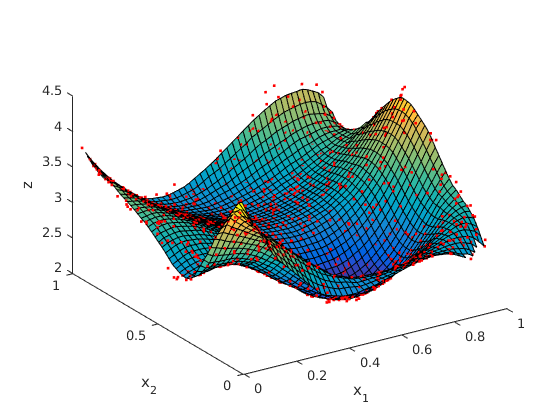
\includegraphics[height=5cm]{figs/train_surface.png}
\end{minipage}%
\begin{minipage}{0.4\textwidth}
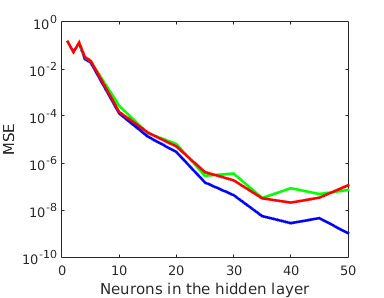
\includegraphics[height=5cm]{figs/performance_val.png}
\end{minipage}
\caption{Left: surface and data points in the training set. Right: Performance on the training, validation and test set as a function of the number of neurons in the hidden layer. \label{fig:performance_val}}
\end{figure}

\begin{figure}[tbh]
\centering
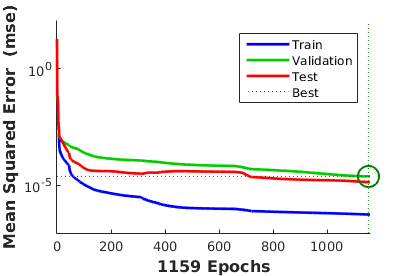
\includegraphics[height=5cm]{figs/MSE_final.png}
\caption{Performance on the training, validation and test set as a function of the number of epochs in the training process. \label{fig:MSE_final}}
\end{figure}

\begin{figure}[tbh]
\centering
\begin{minipage}{0.5\textwidth}
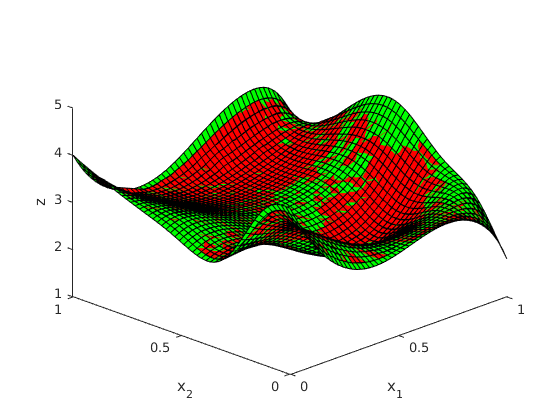
\includegraphics[height=5cm]{figs/NN_and_testsurf.png}
\end{minipage}%
\begin{minipage}{0.5\textwidth}
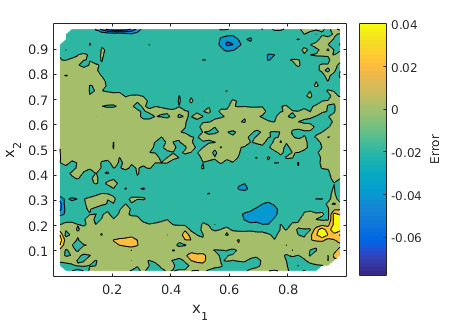
\includegraphics[height=5cm]{figs/NN_test_error.png}
\end{minipage}%
\caption{Left: Neural network (green) and test data (red) surface. The surfaces are almost undistinguishable. Right: Contour plot of the test set error. \label{fig:NN_and_testsurf}}
\end{figure}

To improve the results, we can use all of the provided data, instead of a subset of $3000$. Also, the data division does not need to be equal for all sets. As a rule of thumb, one generally assumes 70:15:15 or 60:20:20 for the train:validation:test set ratios.

\section{Classification of wine data}
Since it is not given whether or not the wine data is linearly separable, we use a non-linear model. We now use a \texttt{tansig} transfer function in the output layer, since this restricts the output to the domain $[-1,1]$ and the target output is in the format of $\pm 1$.
\end{document}